\let\negmedspace\undefined
\let\negthickspace\undefined

\documentclass[journal,12pt,onecolumn]{IEEEtran}
%\documentclass[journal,12pt,twocolumn]{IEEEtran}
%
\usepackage{setspace}
\usepackage{gensymb}
%\doublespacing
\singlespacing

%\usepackage{graphicx}
%\usepackage{amssymb}
%\usepackage{relsize}
\usepackage[cmex10]{amsmath}
%\usepackage{amsthm}
%\interdisplaylinepenalty=2500
%\savesymbol{iint}
%\usepackage{txfonts}
%\restoresymbol{TXF}{iint}
%\usepackage{wasysym}
\usepackage{amsthm}
\usepackage{mathrsfs}
\usepackage{txfonts}
\usepackage{stfloats}
\usepackage{cite}
\usepackage{cases}
\usepackage{subfig}
%\usepackage{xtab}
\usepackage{longtable}
\usepackage{multirow}
%\usepackage{algorithm}
%\usepackage{algpseudocode}
\usepackage{enumitem}
\usepackage{mathtools}
\usepackage{tikz}
\usepackage{circuitikz}
\usepackage{verbatim}
\usepackage{hyperref}
%\usepackage{stmaryrd}
\usepackage{tkz-euclide} % loads  TikZ and tkz-base
%\usetkzobj{all}
\usepackage{listings}
\usepackage{color}                                            %%
\usepackage{array}                                            %%
\usepackage{longtable}                                        %%
\usepackage{calc}                                             %%
\usepackage{multirow}                                         %%
\usepackage{hhline}                                           %%
\usepackage{ifthen}                                           %%
%optionally (for landscape tables embedded in another document): %%
\usepackage{lscape}     
\usepackage{multicol}
\usepackage{chngcntr}
\usepackage{iftex}
%\usepackage[latin9]{inputenc}
\usepackage{geometry}
\usepackage{bm}
%\geometry{verbose,tmargin=2cm,bmargin=3cm,lmargin=1.8cm,rmargin=1.5cm,headheight=2cm,headsep=2cm,footskip=3cm}
\usepackage{array}
\newcolumntype{L}[1]{>{\raggedright\let\newline\\\arraybackslash\hspace{0pt}}m{#1}}
\newcolumntype{C}[1]{>{\centering\let\newline\\\arraybackslash\hspace{0pt}}m{#1}}
\newcolumntype{R}[1]{>{\raggedleft\let\newline\\\arraybackslash\hspace{0pt}}m{#1}}

%\usepackage{graphicx}
%\usepackage{setspace}
%\usepackage{parskip}

\def \hsp {\hspace{3mm}}

\makeatletter

\providecommand{\tabularnewline}{\\}



\makeatother
\ifxetex
\usepackage[T1]{fontenc}
\usepackage{fontspec}
%\setmainfont[ Path = fonts/]{Sanskrit_2003.ttf}
\newfontfamily\nakulafont[Script=Devanagari,AutoFakeBold=2,Path = fonts/]{Nakula}
%\newfontfamily\liberationfont{Liberation Sans Narrow}
%\newfontfamily\liberationsansfont{Liberation Sans}
\fi
\usepackage{tikz}
\usepackage{xcolor}
%\usepackage{enumerate}

%\usepackage{wasysym}
%\newcounter{MYtempeqncnt}
\DeclareMathOperator*{\Res}{Res}
%\renewcommand{\baselinestretch}{2}
\renewcommand\thesection{\arabic{section}}
\renewcommand\thesubsection{\thesection.\arabic{subsection}}
\renewcommand\thesubsubsection{\thesubsection.\arabic{subsubsection}}

\renewcommand\thesectiondis{\arabic{section}}
\renewcommand\thesubsectiondis{\thesectiondis.\arabic{subsection}}
\renewcommand\thesubsubsectiondis{\thesubsectiondis.\arabic{subsubsection}}

% correct bad hyphenation here
\hyphenation{op-tical net-works semi-conduc-tor}
\def\inputGnumericTable{}                                 %%

\lstset{
	language=tex,
	frame=single, 
	breaklines=true
}

%\begin{document}
%


\newtheorem{theorem}{Theorem}[section]
\newtheorem{problem}{Problem}
\newtheorem{proposition}{Proposition}[section]
\newtheorem{lemma}{Lemma}[section]
\newtheorem{corollary}[theorem]{Corollary}
\newtheorem{example}{Example}[section]
\newtheorem{definition}[problem]{Definition}
%\newtheorem{thm}{Theorem}[section] 
%\newtheorem{defn}[thm]{Definition}
%\newtheorem{algorithm}{Algorithm}[section]
%\newtheorem{cor}{Corollary}
\newcommand{\BEQA}{\begin{eqnarray}}
	\newcommand{\EEQA}{\end{eqnarray}}
\newcommand{\define}{\stackrel{\triangle}{=}}
\bibliographystyle{IEEEtran}
%\bibliographystyle{ieeetr}
\providecommand{\mbf}{\mathbf}
\providecommand{\pr}[1]{\ensuremath{\Pr\left(#1\right)}}
\providecommand{\qfunc}[1]{\ensuremath{Q\left(#1\right)}}
\providecommand{\sbrak}[1]{\ensuremath{{}\left[#1\right]}}
\providecommand{\lsbrak}[1]{\ensuremath{{}\left[#1\right.}}
\providecommand{\rsbrak}[1]{\ensuremath{{}\left.#1\right]}}
\providecommand{\brak}[1]{\ensuremath{\left(#1\right)}}
\providecommand{\lbrak}[1]{\ensuremath{\left(#1\right.}}
\providecommand{\rbrak}[1]{\ensuremath{\left.#1\right)}}
\providecommand{\cbrak}[1]{\ensuremath{\left\{#1\right\}}}
\providecommand{\lcbrak}[1]{\ensuremath{\left\{#1\right.}}
\providecommand{\rcbrak}[1]{\ensuremath{\left.#1\right\}}}
\theoremstyle{remark}
\newtheorem{rem}{Remark}
\newcommand{\sgn}{\mathop{\mathrm{sgn}}}
\providecommand{\abs}[1]{\left\vert#1\right\vert}
\providecommand{\res}[1]{\Res\displaylimits_{#1}} 
\providecommand{\norm}[1]{\left\lVert#1\right\rVert}
%\providecommand{\norm}[1]{\lVert#1\rVert}
\providecommand{\mtx}[1]{\mathbf{#1}}
\providecommand{\mean}[1]{E\left[ #1 \right]}
\providecommand{\fourier}{\overset{\mathcal{F}}{ \rightleftharpoons}}
%\providecommand{\hilbert}{\overset{\mathcal{H}}{ \rightleftharpoons}}
%\providecommand{\system}{\overset{\mathcal{H}}{ \longleftrightarrow}}
\providecommand{\system}[1]{\overset{\mathcal{#1}}{ \longleftrightarrow}}
\providecommand{\gauss}[2]{\mathcal{N}\ensuremath{\left(#1,#2\right)}}
%
%\newcommand{\solution}[2]{\textbf{Solution:}{#1}}
\newcommand{\solution}{\noindent \textbf{Solution: }}
\newcommand{\cosec}{\,\text{cosec}\,}
\newcommand{\sinc}{\,\text{sinc}\,}
\newcommand{\rect}{\,\text{rect}\,}
\providecommand{\dec}[2]{\ensuremath{\overset{#1}{\underset{#2}{\gtrless}}}}
\newcommand{\myvec}[1]{\ensuremath{\begin{pmatrix}#1\end{pmatrix}}}
\newcommand{\mydet}[1]{\ensuremath{\begin{vmatrix}#1\end{vmatrix}}}
\newcommand*{\permcomb}[4][0mu]{{{}^{#3}\mkern#1#2_{#4}}}
\newcommand*{\perm}[1][-3mu]{\permcomb[#1]{P}}
\newcommand*{\comb}[1][-1mu]{\permcomb[#1]{C}}
%\numberwithin{equation}{section}
\numberwithin{equation}{section}
%\numberwithin{problem}{section}
%\numberwithin{definition}{section}
\makeatletter
\@addtoreset{figure}{problem}
\makeatother
%\let\StandardTheFigure\thefigure
\let\vec\mathbf
%\renewcommand{\thefigure}{\theproblem.\arabic{figure}}
\renewcommand{\thefigure}{\arabic{section}.\arabic{figure}}
%\setlist[enumerate,1]{before=\renewcommand\theequation{\theenumi.\arabic{equation}}
	%\counterwithin{equation}{enumi}
	%\renewcommand{\theequation}{\arabic{subsection}.\arabic{equation}}
\let\StandardTheFigure\thefigure
	\vspace{3cm}
	%\usepackage{babel}
	\begin{document}
		\title{t-SNE}
		\author{ Mannem Charan AI21BTECH11019}
		 \maketitle
		\begin{abstract}
			This report consists of my basic understanding of one of the modern dimensionality-reduction technique known as "t-SNE".
		\end{abstract}
                \section{t-SNE}
                  t-SNE is a unsupervised learning algorithm used for dimensionality reduction but in general well-suited for visualising the high-dimensional data in low-dimensional space.The full form of t-SNE is t-distributed Stochastic Neighbour Embedding.The idea behind t-SNE is that we will try to find \textbf{similarity scores} in the high-dimensional space between each data point and we will store these values.After that we will try to calculate the similarity scores in low-dimensional space between each data point and then we will compare these set of values with high dimensional space similarity scores.And we will adjust the data points in low-dimensional space such a way these set of scores are as \textbf{similar} as possible.
               \section{Understanding t-SNE}
		  So first we will plot the scatter plot of high-dimensional data.For the sake of simplicity let us take 2-D plot as shown in fig $\ref{2-D}$,
		     \begin{figure}[ht!]
		      \centering
		      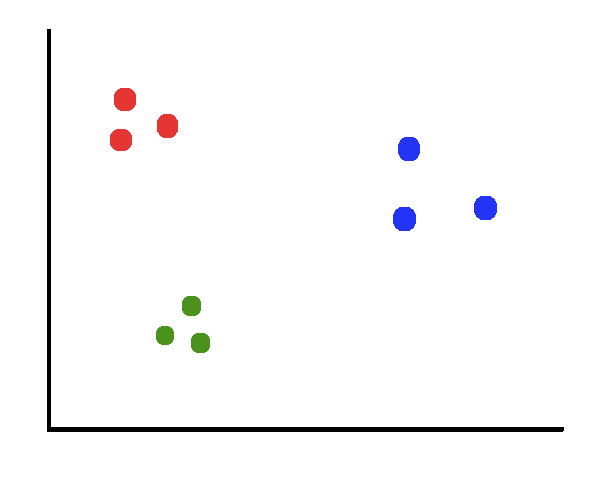
\includegraphics[width = 10cm]{2-D.png}
		      \caption{An example of 2-D dataset}
		      \label{2-D}
	             \end{figure}
		     As you can there are three clusters and we want to convert this 2-D data into a 1-D plot which retains these characteristics$\brak{\text{clusters}}$as shown in figure $\ref{1-D}$,
		     \begin{figure}[ht!]
		      \centering
		      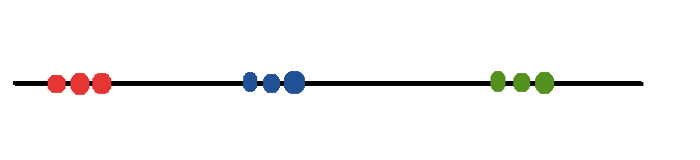
\includegraphics[width = 10cm]{1-D.png}
		      \caption{1-D plot which maintain clear boundaries b/w clusters}
	              \label{1-D}
	             \end{figure}
	       So finding this line in this context is our job. Simply projecting all points on one of the axes will make mess of this data.So to find the line which best represents the data we first need set up some similarity b/w the data points in the orginal data set so that we can use it later.So for that,t-SNE assumes a \textbf{Gaussian distribution} around the target datapoint and the datapoints near to the target datapoint have high likelihood and the datapoints far away has minimum likelihood. And we will renormalize all the likelihood values w.r.t a target datapoint.The reason behind this that sometimes it may happen that the data points in the same cluster$\brak{\text{in case of blue dots}}$ have less density$\brak{\text{the bell curve will be more spread}}$ which leads to low likelihood values in b/w the cluster members.
	       So the values after normalization are what we are calling as \textbf{similarity} values.Mathematically this can be wriiten as,
	        \begin{align}
			p\cbrak{x_j|x_i} &= \frac{\exp\brak{\frac{-\brak{x_j-x_i}^2}{2\sigma_i^2}}}{\sum_{k\neq i}\exp\brak{\frac{-\brak{x_k-x_i}^2}{2\sigma_k^2}}}\label{eq:1}
	        \end{align}
		  where, $p\cbrak{x_j|x_i}$ is the conditional probability that $x_i$ would pick $x_j$ as its neighbour and this value will be the similarity score.\\
Now we will try to find similarity scores of data points in 1-D plot, for that let us take a random line and we will project these data points on the line as shown in the fig $\ref{rand_1-D}$,
		   \begin{figure}[ht!]
		     \centering
		     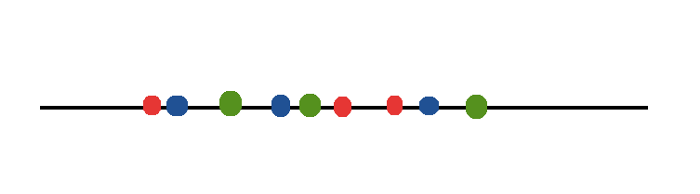
\includegraphics[width = 10cm]{random_positions.png}
		     \caption{Mess}
		     \label{rand_1-D}
		   \end{figure}
	    In this case to find similarity scores we will not use gaussian distribution rather we use a yet another popular distribution known as t-distribution.It is similar to the gaussian distribution but it has heavier tails compared to gaussian.It is employed with this job to make the data look more clear.Similar to earlier we will find the conditional probabilities let say $q\cbrak{x'_j|x'_i}$ where $x'_i$ and $x'_j$ are lower-dimensional counter parts of $x_i$ and $x_j$.\\
	    Now to convert the plot $\ref{rand_1-D}$ to $\ref{1-D}$ we will compare these both distributions using something called Kullback-Liebler divergence$\brak{KL}$.Our goal is to make these similarity scores as close as possible for every pair of data point so that they both map structures the same,to do that we will introduce a cost function which is the sum of these KL divergence over all datapoints.
	    \begin{align}
		    \sum_iKL\brak{P_i||Q_i} &=\sum_i\sum_jp\cbrak{x_j|x_i}\log\frac{p\cbrak{x_j|x_i}}{q\cbrak{x'_j|x'_i}} 
            \end{align}
	    By minimising the cost function SNE retains the local structure $\brak{\text{cluster}}$ of the data in the map.It can be done by using gradient-descent method. The gradient of this cost function looks like,
	    \begin{align}
		    \frac{\partial J}{\partial x'_i} &= 2\sum_{j}\brak{p\cbrak{x_j|x_i} - q\cbrak{x'_j|x'_i} + p\cbrak{x_i|x_j} - q\cbrak{x'_i|x'_j}}
	    \end{align}
	   And the last thing to discuss that the parameter $\sigma_i$ of the gaussian distribution is selected based on how the close the data points in each cluster.So depending on the density at regions we should choose the $\sigma_i$.To find these $\sigma_i$s we will use some called perplexity parameter.This will evaluate the standard deviation for each data point.
	   \section{Questions}
	    \begin{enumerate}
             \item What is the full form of t-SNE?
             \item What is $t$ in t-SNE?
	     \item How the similarity score is calculated in higher dimensional space in t-SNE?
	     \item What is the role of perplexity parameter in SNE?
	     \item What is the main use of t-SNE?
	    \end{enumerate}
	   \section{Answers}
	    \begin{enumerate}
	      \item The full form of t-SNE is t-distributed Stochastic Neighbourhood Embedding.
	      \item The $t$ in t-SNE tells that low-dimensional data takes t-distribution.
	      \item Using eq $\eqref{eq:1}$ we can calculate the similarity score in high dimensional space.
	      \item The perpelexity parameter controls the number of neighbours the datapoint can have and it is a tuneable parameter.
	      \item t-SNE is used to understand the high dimensional data and project it into low dimensional data.It is more used data visualisation rather as a data preprocessing step.
	    \end{enumerate}
        \end{document}




